%%%%%%%%%%%%%%%%%%%%%%%%%%%%%%%%%%%%%%%%%%%%%%%%%%%%%%%%%%%%%%%%%%%%%%%%%%%%%%%%
%%                                                                
%%      SWSC LaTeX class for Journal of Space Weather and Space Climate
%%      
%%                                      (c) Springer-Verlag HD
%%                                      revised by EDP Sciences
%%                                      further revised by J. Watermann 
%%
%%%%%%%%%%%%%%%%%%%%%%%%%%%%%%%%%%%%%%%%%%%%%%%%%%%%%%%%%%%%%%%%%%%%%%%%%%%%%%%%
%%
%%      This demonstration file was derived from aa.dem
%%  
%%      AA vers. 7.0, LaTeX class for Astronomy & Astrophysics
%%      demonstration file
%%                                                (c) Springer-Verlag HD
%%                                                revised by EDP Sciences
%%
%%%%%%%%%%%%%%%%%%%%%%%%%%%%%%%%%%%%%%%%%%%%%%%%%%%%%%%%%%%%%%%%%%%%%%%%%%%%%%%%
%%
%%      modified for Journal of Space Weather and Space Climate
%%      by Jurgen Watermann, Editorial Advisor to SWSC
%%
%%      01-04-2012
%%      02-04-2012 revision 1
%%      12-07-2012 revision 2
%%      06-12-2012 revision 3 
%%      01-01-2014 revision 4
%%      06-03-2014 revision 4.1
%%
%%%%%%%%%%%%%%%%%%%%%%%%%%%%%%%%%%%%%%%%%%%%%%%%%%%%%%%%%%%%%%%%%%%%%%%%%%%%%%%%
%%
%%      The two sub-figures referenced in this template are of eps and png type,
%%      respectively, in order to demonstrate the usepackages subfigure and
%%      epstopdf and thus create pdf-only output 
%%
%%      If you want to use TexLive or MikTex together with a bibtex bibliography 
%%      file you may run Latex2e from the command line 
%%          pdflatex -shell-escape swsc.tex
%%          bibtex swsc (do not include an extension such as .tex or .bib)
%%          pdflatex -shell-escape swsc.tex
%%          pdflatex -shell-escape swsc.tex
%%
%%      A double call to pdflatex after calling bibtex is necessary in order to
%%      set citations and references correctly and insure that foreward/backward  
%%      linkage (backref option) is properly applied
%%      If you use MikTex you may need to make a triple call to pdflatex
%%
%%      If you are using TexLive or MikTex but not a bibtex type of bibliography
%%      you may simply run Latex2e twice from the command line 
%%          pdflatex -shell-escape swsc.tex
%%          pdflatex -shell-escape swsc.tex
%%
%%%%%%%%%%%%%%%%%%%%%%%%%%%%%%%%%%%%%%%%%%%%%%%%%%%%%%%%%%%%%%%%%%%%%%%%%%%%%%%%
%%
%%   single column 12-point version for review
%%

%%  with traditional abstract
\documentclass[referee,a4paper,12pt,traditabstract]{swsc} 

%%  with structured abstract 
%\documentclass[referee,a4paper,12pt,structabstract]{swsc} 

\usepackage{graphicx}
\usepackage{txfonts}
\usepackage{subfigure}
\usepackage{epstopdf}
\usepackage{lineno}
\usepackage[authoryear,round]{natbib}
\usepackage[backref]{hyperref}
\usepackage{url}
\usepackage[inline]{enumitem}
\usepackage{verbatim}
%%    This version assumes using bibtex with the swsc bibliography style file
\bibliographystyle{swsc.bst}

\hypersetup{colorlinks=true,citecolor=cyan,urlcolor=cyan,linkcolor=blue}

%%%%%%%%%%%%%%%%%%%%%%%%%%%%%%%%%%%%%%%%%%%%%%%%%%%%%%%%%%%%%%%%%%%%%%%%%%%%%%%%

\begin{document}

\begin{linenumbers}

   \title{Gaussian Processes Autoregressive Models for Forecasting the Disturbance Storm Time Index}

   \titlerunning{Gaussian Process $Dst$ models}

   \authorrunning{Chandorkar et. al}

   \author{M. Chandorkar
          \inst{1}
          \and
          E. Camporeale\inst{1}
          \and 
          S. Wing \inst{2}
          }

   \institute{\inst{1} Centrum Wiskunde Informatica (CWI), Amsterdam,
              1098XG Amsterdam\\
              \ \email{\href{mailto:m.h.chandorkar@cwi.nl}{m.h.chandorkar@cwi.nl} \href{mailto:e.camporeale@cwi.nl}{e.camporeale@cwi.nl}}\\
              \inst{2} The Johns Hopkins University Applied Physics Laboratory, 
              Laurel, Maryland, 20723, USA
             }
               
   

%%   \date{Received September 15, 1996; accepted March 16, 1997}

  % \abstract{}{}{}{}{}        %% uncomment if structured abstract is desired
 %% 5 {} token are mandatory
 
   %% replace by pair of curly brackets, {}, if structured abstract is selected
   
   
   \abstract{
    We present two models, based on Gaussian Processes, for the \emph{One Step Ahead}(OSA) prediction of the $Dst$ geomagnetic activity index. 
    The models are Auto regressive, with or without eXogenous inputs (GP-ARX and GP-AR, respectively).
    We compare the performance of these models with the current state of the art in one step ahead $Dst$ prediction on a set of 
    63 benchmark storms from 1998-2006, previously analyzed in an earlier study.
    We show that, despite its lack of sophistication, the so-called Persistence model represents an important test to evaluate the performance of a one hour ahead $Dst$ model.
    Contrary to the state-of-the-art models compared in the literature, our models consistently outperform the Persistence model and represent a substantial improvement in the field, when evaluated on standard metrics.
    Finally, an important feature of the new models is that they naturally provide confidence intervals for their forecast.
    }

   \keywords{Geomagnetic indices --
            $Dst$ OSA Prediction --
            Gaussian Processes --
            Machine Learning
            }

   \maketitle
%%
%%________________________________________________________________

\section{Introduction}

The magnetosphere's dynamics and its associated solar wind driver form a complex dynamical system. It is therefore instructive and greatly simplifying to use representative indices to quantify the state of geomagnetic activity.

Geomagnetic indices come in various forms, they may take continuous or discrete values and may be defined with varying time resolutions. Their values are often calculated by averaging or combining a number of readings taken by instruments around the Earth. Each geomagnetic index is a proxy for a particular kind of phenomenon. Some popular indices are the $K_p$, $Dst$ and the $AE$ index.

\begin{enumerate}
    \item $K_p$: The Kp-index is a discrete valued global geomagnetic storm index and is based on 3 hour measurements of the K-indices \citep{Bartels}. The K-index itself is a three hour long quasi-logarithmic local index of the geomagnetic activity, relative to a calm day curve for the given location.
    
    \item $AE$: The Auroral Electrojet Index, $AE$, is designed to provide a global, quantitative measure of auroral zone magnetic activity produced by enhanced Ionospheric currents flowing below and within the auroral oval \citep{AEIndex}. It is a continuous index which is calculated every hour.
    
    \item $Dst$: A continuous hourly index which measures the weakening of the Earths magnetic field due to ring currents and the strength of geomagnetic storms \citep{DesslerAndParker}. 
\end{enumerate}

%Talk about Burton and friends
For the present study, we focus on prediction of the hourly $Dst$ index which is a straightforward indicator of geomagnetic storms. More specifically, we focus on the \emph{one step ahead} (OSA), in this case one hour ahead prediction of $Dst$ because it is the simplest model towards building long term predictions of geomagnetic response of the Earth to changing space weather conditions. 

The $Dst$ OSA prediction problem has been the subject of several modeling efforts in the literature. One of the earliest models has been presented by \citet{JGR:JGR10260} who calculated $Dst(t)$ as the solution of an \emph{Ordinary Differential Equation} (ODE) which expressed the rate of change of $Dst(t)$ as a combination of two terms: decay and injection $\frac{d Dst(t)}{dt} = Q(t) - \frac{Dst(t)}{\tau}$, where Q(t) relates to the particle injection from the plasma sheet into the inner magnetosphere. 

The \citet{JGR:JGR10260} model has proven to be very influential particularly due to its simplicity. Many subsequent works have modified the proposed ODE by proposing alternative expressions for the injection term $Q(t)$ [see \citet{Wang:Dst}, \citet{JGRA:JGRA14856}]. More recently \citet{Ballatore2014} have tried to generate empirical estimates for the injection and decay terms in Burton's equation.

%Talk about NARMAX Dst
Another important empirical model used to predict $Dst$ is the \emph{Nonlinear Auto-Regessive Moving Average with eXogenous inputs} (NARMAX) methodology developed in \citet{doi:10.1080/00207178908559767}, \citet{GRL:GRL13494}, \citet{GRL:GRL20944}, \citet{JGRA:JGRA18657}, \citet{balikhin:narmax}, \citet{JGRA:JGRA20661} and \citet{JGRA:JGRA50192}. The NARMAX methodology builds models by constructing polynomial expansions of inputs and determines the best combinations of monomials to include in the refined model by using a criterion called the \emph{error reduction ratio} (ERR). The parameters of the so called NARMAX OLS-ERR model are calculated by solving the \emph{ordinary least squares} (OLS) problem arising from a quadratic objective objective function. The reader may refer to \citet{billings2013nonlinear} for a detailed exposition of the NARMAX methodology.

%Talk about neural networks
Yet another family of forecasting methods is based on \emph{Artificial Neural Networks} (ANN) that have been a popular choice for building predictive models. Researchers have employed both the standard \emph{feed forward} and the more specialized \emph{recurrent} architectures. \citet{Lund} proposed an \emph{Elman} recurrent network architecture called Lund $Dst$, which used the solar wind velocity, \emph{interplanetary magnetic field} (IMF) and historical $Dst$ data as inputs. \citet{JGRA:JGRA17461} used recurrent neural networks to predict $Kp$. \citet{SWE:SWE286} originally proposed a \emph{feed forward} network for predicting the $K_p$ index which used the \emph{Boyle coupling function} \citep{boyle1997empirical}. The same architecture is adapted for prediction of $Dst$ in \citet{SWE:SWE286}, popularly known as the Rice $Dst$ model. \citet{pallocchia:hal-00318011} proposed a \emph{neural network} model called EDDA to predict $Dst$ using only the IMF data.

%Talk about comparison papers, number of storms covered and Persistence
In light of the extensive list of modeling techniques employed for prediction of the $Dst$ index, model comparison and evaluation becomes a crucial step for advancing the research domain. \citet{Rastatter2013} compared several physics based (convection, kinetic and magneto hydrodynamic) and empirical prediction models such as NARMAX, Rice $Dst$ on 4 storm events which occurred between 2001 and 2006. \citet{Amata2008} compared the EDDA and the Lund $Dst$ models over the 2003-2005 period. The most extensive model comparison in terms of storm events was probably conducted in \citet{Ji2012} which compared six $Dst$ models (see table \ref{table:DstModels}) on a list of 63 geomagnetic storm events of varying intensities which occurred between 1998 and 2006. In the comparison done in \citet{Ji2012}, the model proposed in \citet{JGRA:JGRA16300} gives the best performance on the test set considered. 

%Vision
In $Dst$ prediction, a seemingly trivial yet highly informative prediction method is represented by the so called \emph{Persistence} model, which uses the previous value of $Dst$ as the prediction for the next time step ($\hat{D}st(t) = Dst(t-1)$). Due to high correlation between $Dst$ values one hour apart ($Dst(t)$, $Dst(t-1)$), the \emph{Persistence} model gives excellent predictive performance on error metrics, despite its apparent lack of sophistication. In essence it is a trivial hypothesis and hence it should always be used as a base line to compare the performance of any proposed $Dst$ algorithm. Moreover, given its zero computational cost, a model should at least outperform the \emph{Persistence} model in order to be a viable candidate for advancing the science of space weather prediction. An obvious critique to the Persistence model is that it is not really predictive, in the sense that it cannot forecast a storm, until it has already commenced. However, most of the literature has used global metrics, such as the Root Mean Square Error (RMSE, see section \ref{sec:exp}) to evaluate models. It is in this context that we argue that the Persistence model should be regarded as the first candidate to outperform.

%Assertion
In this paper, we propose \emph{Gaussian Process} models for OSA prediction of $Dst$. We use the results of \citet{Ji2012} as a starting point and compare our proposed models with the methods evaluated in that paper, while using the performance of the \emph{Persistence} model as a base line. 

% Talk about Gaussian Process
We use hourly resolution measurements extracted from NASA/GSFC's OMNI data set through OMNIWeb \citep{OmniPaper}. The rest of the paper is organized as follows. Section \ref{sec:method} gives an introduction to the \emph{Gaussian Process} methodology for regression and some technical details about their application. In section \ref{sec:osa} two different \emph{Gaussian Process} auto-regressive models are proposed and subsequently in sections \ref{sec:exp} and \ref{sec:res}, bench marked against the \emph{Persistence} as well as the other models outlined in \citet{Ji2012}.

  
\section{Methodology: Gaussian Process} \label{sec:method}

\emph{Gaussian Processes} first appeared in machine learning research in \citet{Neal:1996:BLN:525544}, as the limiting case of Bayesian inference performed on neural networks with infinitely many neurons in the hidden layers. Although their inception in the machine learning community is recent, their origins can be traced back to the geo-statistics research community where they are known as \emph{Kriging} methods (\citet{krige1951statistical}). In pure mathematics area \emph{Gaussian Processes} have been studied extensively and their existence was first proven by Kolmogorov's extension theorem (\citet{tao2011introduction}). The reader is referred to \cite{Rasmussen:2005:GPM:1162254} for an in depth treatment of Gaussian Processes in machine learning.

Let us assume that we want to model a process in which a scalar quantity $y$ is described by $y = f(\mathbf{x}) + \epsilon$ where   $f(.): \mathbb{R}^d \rightarrow \mathbb{R}$ is an unknown scalar function of a multidimensional input vector $\mathbf{x} \in \mathbb{R}^d$, and $\epsilon \sim \mathcal{N}(0, \sigma^2)$ is Gaussian distributed noise with variance $\sigma^2$.

A set of labeled data points ${(\mathbf{x}_i, y_i); i = 1 \cdots N}$ can be conveniently expressed by a $N \times d$ data matrix $\mathbf{X}$ and a $N \times 1$ response vector $\mathbf{y}$, as shown in equations (\ref{eq:feat}) and (\ref{eq:labels}).

\begin{eqnarray}
  \mathbf{X} & = & \left( \begin{array}{c} \mathbf{x}^{T}_1 \\ \mathbf{x}^{T}_2 \\ \vdots \\ \mathbf{x}^{T}_n \end{array} \right)_{n \times d} \label{eq:feat} \\
  \vspace{2\baselineskip}
  \mathbf{y} & = & \left( \begin{array}{c} y_1 \\ y_2 \\ \vdots \\ y_N \end{array} \right) _{n \times 1} \label{eq:labels}
\end{eqnarray}

Our task is to infer the values of the unknown function $f(.)$ based on the inputs $\mathbf{X}$ and the noisy observations $\mathbf{y}$. We now assume that the joint distribution of $f(\mathbf{x}_i), i = 1 \cdots N$ is a multivariate Gaussian as shown in equations (\ref{eq:fvalues}), (\ref{eq:normal}) and (\ref{eq:sto}).

\begin{eqnarray}
 \mathbf{f} & = & \left( \begin{array}{c} f(\mathbf{x}_1) \\ f(\mathbf{x}_2) \\ \vdots \\ f(\mathbf{x}_N) \end{array} \right) \label{eq:fvalues}\\
 \vspace{2\baselineskip}
 \mathbf{f} | \mathbf{x}_1, \cdots, \mathbf{x}_N & \sim & \mathcal{N}\left( \mathbf{\mu}, \mathbf{\Lambda} \right)  \label{eq:normal}\\
 \vspace{2\baselineskip}
 p( \mathbf{f} \ | \ \mathbf{x}_1, \cdots, \mathbf{x}_N) & = & \frac{1}{(2\pi)^{n/2} det(\mathbf{\Lambda})^{1/2}} exp \left(-\frac{1}{2} (\mathbf{f} - \mathbf{\mu})^T \mathbf{\Lambda}^{-1} (\mathbf{f} - \mathbf{\mu}) \right) \label{eq:sto}
\end{eqnarray}

Here $\mathbf{f}$ is a $N\times 1$ vector consisting of the values $f(\mathbf{x}_i), i = 1 \cdots N$. In equation (\ref{eq:normal}), $\mathbf{f}|\mathbf{x}_1, \cdots, \mathbf{x}_N$ denotes the conditional distribution of $\mathbf{f}$ with respect to the input data (i.e., $\mathbf{X}$) and $\mathcal{N}\left( \mathbf{\mu}, \mathbf{\Lambda} \right)$ represents a multivariate Gaussian distribution with mean vector $\mathbf{\mu}$ and covariance matrix $\mathbf{\Lambda}$. The probability density function of this distribution $p( \mathbf{f} \ | \ \mathbf{x}_1, \cdots, \mathbf{x}_N)$ is therefore given by equation (\ref{eq:sto}).

From equation (\ref{eq:sto}), one can observe that in order to uniquely define the distribution of the process, it is required to specify $\mathbf{\mu}$ and $\mathbf{\Lambda}$. For this probability density to be valid, there are further requirements imposed on $\mathbf{\Lambda}$: 

\begin{enumerate}
      \item Symmetry: $\mathbf{\Lambda}_{ij} = \mathbf{\Lambda}_{ji} \ \forall i,j \in {1, \cdots, N} $ 
      \item Positive Semi-definiteness: $\mathbf{z}^T \mathbf{\Lambda} \mathbf{z} \geq 0 \ \forall \mathbf{z} \in \mathbb{R}^N$  
\end{enumerate}

Inspecting the individual elements of $\mathbf{\mu}$ and $\mathbf{\Lambda}$, we realise that they take the following form.

\begin{eqnarray}
      \mu_i & = & \mathbb{E}[f(\mathbf{x}_i)] := m(\mathbf{x}_i) \\
      \Lambda_{ij} & = & \mathbb{E}[(f(\mathbf{x}_i) - \mu_i)(f(\mathbf{x}_j) - \mu_j)] := K(\mathbf{x}_i, \mathbf{x}_j)
\end{eqnarray}

Here $\mathbb{E}$ denotes the expectation (average). The elements of $\mathbf{\mu}$ and $\mathbf{\Lambda}$ are expressed as functions $m(\mathbf{x}_i)$ and $K(\mathbf{x}_i, \mathbf{x}_j)$ of the inputs $\mathbf{x}_i,\ \mathbf{x}_j$. Specifying the functions $m(\mathbf{x})$ and $K(\mathbf{x}, \mathbf{x}')$ completely specifies each element of $\mathbf{\mu}$ and $\mathbf{\Lambda}$ and subsequently the finite dimensional distribution of $\mathbf{f} | \mathbf{x}_1, \cdots, \mathbf{x}_N $. In most practical applications of \emph{Gaussian Processes} the mean function is often defined as $m(\mathbf{x}) = 0$, which is not unreasonable if the data is standardized to have zero mean. \emph{Gaussian Processes} are represented in machine learning literature using the following notation:

\begin{equation}
    f(\mathbf{x}) \sim \mathcal{GP}(m(\mathbf{x}), K(\mathbf{x}, \mathbf{x}'))
\end{equation}

\subsection{Inference and Predictions} \label{sec:inference}

Our aim is to infer the function $f(\mathbf{x})$ from the noisy training data and generate predictions $f(\mathbf{x}^{*}_i)$ for a set of test points $ {\mathbf{x}^{*}_i : \forall i \in 1, \cdots, M} $. We define $\mathbf{X}^*$ as the test data matrix whose rows are formed by $\mathbf{x}^{*}_i$ as shown in equation (\ref{eq:testfeat}). 
\begin{equation}
    \mathbf{X}_* = \left( \begin{array}{c} (\mathbf{x}^{*}_1)^T \\ (\mathbf{x}^{*}_2)^T \\ \vdots \\ (\mathbf{x}^{*}_M)^T \end{array} \right)_{M \times d} \label{eq:testfeat} 
\end{equation}
Using the multivariate Gaussian distribution in equation (\ref{eq:sto}) we can construct the joint distribution of $f(\mathbf{x})$ over the training and test points. The vector of training and test outputs $\left( \begin{array}{c} \mathbf{y} \\ \mathbf{f_*} \end{array} \right)$ is of dimension $(N+M) \times 1$ and is constructed by appending the test set predictions $\mathbf{f}_*$ to the observed noisy measurements $\mathbf{y}$.

\begin{eqnarray}
    \mathbf{f}_* & = & \left( \begin{array}{c} f(\mathbf{x^{*}_1}) \\ f(\mathbf{x^{*}_2}) \\ \vdots \\ f(\mathbf{x^{*}_M}) \end{array} \right)_{M \times 1} \\
     \vspace{4\baselineskip}
    \left( \begin{array}{c} \mathbf{y} \\ \mathbf{f_*} \end{array} \right) | \ \ \mathbf{X}, \mathbf{X}_* & \sim & 
    \mathcal{N}\left(\mathbf{0}, \left[ \begin{array}{cc} \mathbf{K} + \sigma^{2} \mathbf{I} & \mathbf{K}_{*} \\ \mathbf{K}_{*}^T & \mathbf{K}_{**} \end{array} \right ] \right) \label{eq:dist}
\end{eqnarray}

Since we have noisy measurements of $f$ over the training data, we add the noise variance $\sigma^2$ to the variance of $f$ as shown in (\ref{eq:dist}). The block matrix components of the $(N+M) \times (N+M)$ covariance matrix have the following structure.

\begin{enumerate}
      \item $\mathbf{I}$: The $n \times n$ identity matrix.
      \item $\mathbf{K} = [K(\mathbf{x}_i, \mathbf{x}_j)], \ i,j \in 1,\cdots,n$ : Kernel matrix constructed from all couples obtained from the training data.
      \item $\mathbf{K}_{*} = [K(\mathbf{x}_i, \mathbf{x}^{*}_j)], \ i \in 1,\cdots,n ; j \in 1,\cdots,m$ : Cross kernel matrix constructed from all couples between training and test data points.
      \item $\mathbf{K}_{**} = [K(\mathbf{x}^{*}_i, \mathbf{x}^{*}_j)], \ i,j \in 1,\cdots,m$: Kernel matrix constructed from all couples obtained from the test data.
\end{enumerate}

With the multivariate normal distribution defined in equation (\ref{eq:dist}), probabilistic predictions $f_*$ can be generated by constructing the conditional distribution $\mathbf{f_*}|\mathbf{X},\mathbf{y},\mathbf{X_*}$. Since the original distribution of $\left( \begin{array}{c} \mathbf{y} \\ \mathbf{f_*} \end{array} \right) | \ \ \mathbf{X}, \mathbf{X}_*$ is a multivariate Gaussian, conditioning on a subset of elements: $\mathbf{y}$ yields another Gaussian distribution whose mean and covariance can be calculated exactly, as in equation (\ref{eq:posterior}) (see \citet{Rasmussen:2005:GPM:1162254}).
\begin{equation}
    \mathbf{f_*}|\mathbf{X},\mathbf{y},\mathbf{X_*} \sim \mathcal{N}(\mathbf{\bar{f}_*}, \Sigma_*)  \label{eq:posterior},
\end{equation}
where
\begin{eqnarray}
    \mathbf{\bar{f}_*} & = & \mathbf{K}^T_{*} [\mathbf{K} + \sigma^{2} \mathbf{I}]^{-1} \mathbf{y} \label{eq:posteriormean} \\
    \Sigma_* & = & \mathbf{K}_{**} - \mathbf{K}^T_{*} \left(\mathbf{K} + \sigma^{2} \mathbf{I}\right)^{-1} \mathbf{K}_{*} \label{eq:posteriorcov}
\end{eqnarray}

The practical implementation of \emph{Gaussian Process} models requires the inversion of the training data kernel matrix $[\mathbf{K} + \sigma^{2} \mathbf{I}]^{-1}$ to calculate the parameters of the predictive distribution $\mathbf{f_*}|\mathbf{X},\mathbf{y},\mathbf{X_*}$. The computational complexity of this inference is dominated by the linear problem $\mathbf{K}^T_{*} [\mathbf{K} + \sigma^{2} \mathbf{I}]^{-1} \mathbf{y}$, which can be solved via Cholesky decomposition, with a time complexity of $O(N^3)$, where $N$ is the number of data points.

The distribution of $\mathbf{f_*}| \mathbf{X},\mathbf{y},\mathbf{X_*}$ is known in Bayesian analysis as the \emph{Posterior Predictive Distribution}. This illustrates a key difference between \emph{Gaussian Processes} and other regression models such as \emph{Neural Networks}, \emph{Linear Models} and \emph{Support Vector Machines}: a \emph{Gaussian Process} model does not generate point predictions for new data but outputs a predictive distribution for the quantity sought, thus allowing to construct error bars on the predictions. This property of Bayesian models such as \emph{Gaussian Processes} makes them very appealing for Space Weather forecasting applications. 

The central design issue in applying \emph{Gaussian Process} models is the choice of the function $K(\mathbf{x}, \mathbf{x}')$. The same constraints that apply to $\mathbf{\Lambda}$ also apply to the function $K$. In machine learning, these symmetric positive definite functions of two variables are known as \emph{kernels}. Kernel based methods are applied extensively in data analysis i.e. regression, clustering, classification, density estimation (see \citet{Scholkopf:2001:LKS:559923}, \citet{hofmann2008}).

\subsection{Kernel Functions}

For the success of a \emph{Gaussian Process} model an appropriate choice of kernel function is paramount. The symmetry and positive semi-definiteness of \emph{Gaussian Process} kernels implies that they represent inner-products between some basis function representation of the data. The interested reader is suggested to refer to \cite{Berlinet2004}, \citet{Scholkopf:2001:LKS:559923} and \citet{hofmann2008} for a thorough treatment of kernel functions and the rich theory behind them. Some common kernel functions used in machine learning include the radial basis function (RBF) kernel $K(\mathbf{x}, \mathbf{y}) = \frac{1}{2} exp(-||\mathbf{x} - \mathbf{y}||^2/l^2)$ and the polynomial kernel $K(\mathbf{x}, \mathbf{y}) = (\mathbf{x}^\intercal \mathbf{y} + b)^d$. 

The quantities $l$ in the RBF, and $b$ and $d$ in the polynomial kernel are known as \emph{hyper-parameters}. Hyper-parameters give flexibility to particular kernel structure, for example $d = 1, 2, 3, \cdots$ in the polynomial kernel represents linear, quadratic, cubic and higher order polynomials respectively. The method of assigning values to the \emph{hyper-parameters} is crucial in the model building process. 

In this study, we construct Gaussian Process regression models with linear kernels as shown in equation (\ref{eq:usedKernel}), for \emph{one step ahead} prediction of the $Dst$ index. Our choice of kernel leaves us with only one adjustable hyper-parameter, the model noise $\sigma$. 

\begin{equation}\label{eq:usedKernel}
    K(\mathbf{x}, \mathbf{y}) = \mathbf{x}^\intercal \mathbf{y}
\end{equation}

We initialize a grid of values for the model noise $\sigma$ and use the error on a predefined validation data set to choose the best performing value of $\sigma$. While constructing the grid of possible values for $\sigma$ it must be ensured that $\sigma > 0$ so that the kernel matrix constructed on the training data is non-singular.

\section{One Step Ahead Prediction} \label{sec:osa}

Below in equations (\ref{eq:Dst}) - (\ref{eq:GPPoly}) we outline a \emph{Gaussian Process} formulation for \emph{OSA} prediction of $Dst$. A vector of features $x_{t-1}$ is used as input to an unknown function $f(x_{t-1})$.

The features $x_{t-1}$ can be any collection of quantities in the hourly resolution OMNI data set. Generally $x_{t-1}$ are time histories of $Dst$ and other important variables such as plasma pressure $p(t)$, solar wind speed $V(t)$, z component of the interplanetary magnetic field $B_z(t)$.

\begin{eqnarray}
    Dst(t) & = & f(\mathbf{x}_{t-1}) + \epsilon \label{eq:Dst} \\
    \epsilon & \sim & \mathcal{N}(0, \sigma^2) \label{eq:GPNoise} \\
    f(x_t) & \sim & \mathcal{GP}(m(\mathbf{x}_t), K(\mathbf{x}_t, \mathbf{x}_s)) \label{eq:DstGP} \\
    K(\mathbf{x}, \mathbf{y}) & = & \mathbf{x}^\intercal \mathbf{y} + b \label{eq:GPPoly}
\end{eqnarray}

In the following we consider two choices for the input features $\mathbf{x}_{t-1}$ leading to two variants of \emph{Gaussian Process} regression for $Dst$ time series prediction.

\subsection{Gaussian Process Auto-Regressive (GP-AR)} \label{sec:gpar}

The simplest auto-regressive models for \emph{OSA} prediction of $Dst$ are those that use only the history of $Dst$ to construct input features for model training. The input features $\mathbf{x}_{t-1}$ at each time step are the history of $Dst(t)$ until a time lag of $p$ hours.

\begin{eqnarray*}
    \mathbf{x}_{t-1} & = & \left(Dst(t-1), \cdots , Dst(t-p+1)\right)
\end{eqnarray*}

\subsection{Gaussian Process Auto-Regressive with eXogenous inputs (GP-ARX)} \label{sec:gparx}

Auto-regressive models can be augmented by including exogenous quantities in the inputs $\mathbf{x}_{t-1}$ at each time step, in order to improve predictive accuracy. $Dst$ gives a measure of ring currents, which are modulated by plasma sheet particle injections into the inner magnetosphere during sub-storms. Studies have shown that the substorm occurrence rate increases with solar wind velocity (high speed streams) \citep{Kissinger2011,Newell2016}. Prolonged southward interplanetary magnetic field (IMF) z-component ($B_z$) is needed for sub-storms to occur \citep{McPherron1986}. An increase in the solar wind electric field, $VB_z$, can increase the dawn-dusk electric field in the magnetotail, which in turn determines the amount of plasma sheet particle that move to the inner magnetosphere \citep{Friedel2001}. Therefore, our exogenous parameters consist of solar wind velocity, IMF $B_z$, and $VB_z$.   

In this model we choose distinct time lags $p$ and $p_{ex}$ for auto-regressive and exogenous variables respectively. In addition we explicitly include the product $V B_z$ which is a proxy for the electric field, as an input.
    
\begin{eqnarray*}
        & \mathbf{x}_{t-1} & = (Dst(t-1), \cdots , Dst(t-p+1), \\
        & \ \ \ \ \ & V(t-1), \cdots, V(t-p_{ex}+1),\\
        & \ \ \ \ \ & B_{z}(t-1), \cdots, B_{z}(t-p_{ex}+1),\\
        & \ \ \ \ \ & V B_{z}(t-1), \cdots, V B_{z}(t-p_{ex}+1))
\end{eqnarray*}

\section{Model Training and Validation}

Before running performance bench marks for \emph{OSA} $Dst$ prediction on the storm events in \cite{Ji2012}, training and model selection of \emph{GP-AR} and \emph{GP-ARX} models on independent data sets must be performed. For this purpose we choose segments 00:00 1 January 2008 - 10:00 11 January 2008 for training and 00:00 15 November 2014 - 23:00 1 December 2014 for model selection. 

Although the training and model selection data sets both do not have a geomagnetic storm in them, this would not degrade the performance of \emph{GP-AR} and \emph{GP-ARX} because the linear polynomial kernel describes a non stationary and self similar Gaussian Process. This implies that for two events where the time histories of $Dst$, $V$ and $B_z$ are not close to each other but can be expressed as a diagonal rescaling of time histories observed in the training data, the predictive distribution is a linearly rescaled version of the training data $Dst$ distribution. 

The computational complexity of calculation of the predictive distribution is $O(N^3)$ as per section \label{sec:inference} this can limit the size of the covariance matrix constructed from the training data. Note that this computation overhead is paid for every unique assignment to the model hyper-parameters.

Model selection of \emph{GP-AR} and \emph{GP-ARX} is performed by grid search methodology and the root mean square error (\emph{RMSE}) on the validation set is used to select the values of the model hyper-parameters. In the experiments performed the best performing values of the hyper-parameters outputted by the grid search routine are $\sigma = 0.45$ for the \emph{GP-ARX} and $\sigma = 1.173$ for \emph{GP-AR}. 

The time lags chosen for \emph{GP-AR} are $p = 6$ while for \emph{GP-ARX} $p=6$, $p_{ex} = 1$ are arrived by experimenting with values starting from one and choosing the value of $p$ yielding best performance on the 63 events in the bench mark. We do not feel that this approach for choosing the time lags leads to bias towards models which only perform well on the data set of \citet{Ji2012} because Gaussian Processes are not easily susceptible to overfitting for situations when the number of model hyper-parameters is small or leave one out cross-validation is not performed.

\begin{figure}
   \centering
   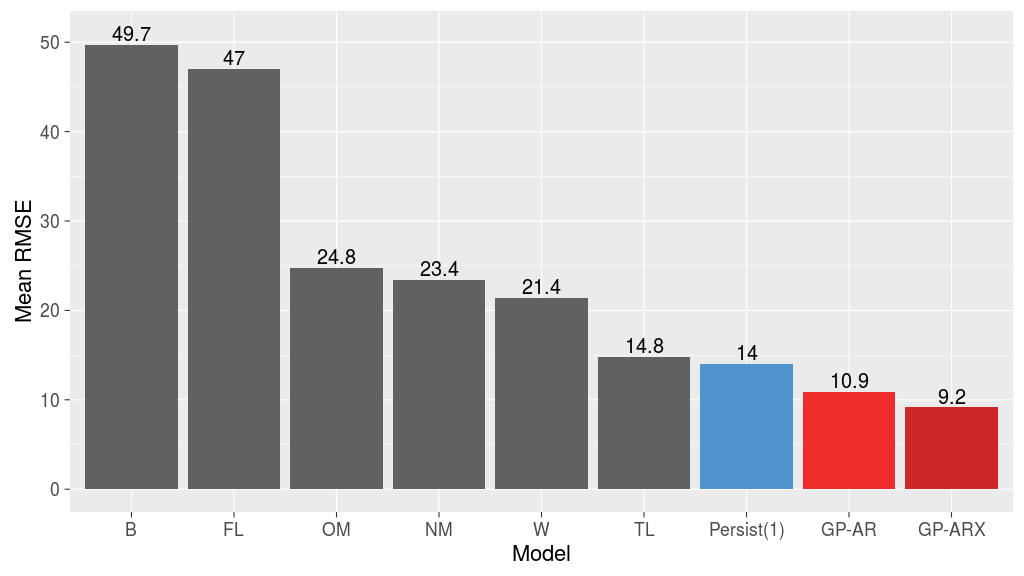
\includegraphics[width=\textwidth]{Compare_RMSE.png}
      \caption{Averaged RMSE performance of \emph{GP-AR}, \emph{GP-ARX} and the \emph{Persistence} model versus results in \citet{Ji2012}.}
         \label{fig:rmse}
   \end{figure}

\section{Experiments} \label{sec:exp}

\citet{Ji2012} compare six \emph{one step ahead} $Dst$ models as listed in table \ref{table:DstModels} in their paper by compiling a list of 63 geomagnetic storm events of varying strengths which occurred in the period 1998-2006. This serves as an important stepping stone for a systematic comparison of existing and new prediction techniques because performance metrics are averaged over a large number of storm events that occurred over a 8 year period. They compare the averaged performance of these models on four key performance metrics.

\begin{enumerate}
    \item The root mean square error.
    \begin{equation}
        RMSE = \sqrt{\sum_{t=1}^{n} (Dst(t) - \hat{D}st(t))^2 / n}
    \end{equation}
    \item Correlation coefficient between the predicted and actual value of $Dst$.
    \begin{equation}
        CC = Cov(Dst, \hat{D}st)/\sqrt{Var(Dst) Var(\hat{D}st)}
    \end{equation}
    \item The error in prediction of the peak negative value of $Dst$ for a storm event.
    \begin{equation}
        \Delta Dst_{min} = Dst(t^*) - \hat{D}st(t^{**}), \ t^* = argmin(Dst(t)),\ t^{**} = argmin(\hat{D}st(t))
    \end{equation}
    \item The error in predicting the timing of a storm peak, also called \emph{timing error} $|\Delta t_{peak}|$.
    \begin{equation}
        \Delta t_{peak} = \mathit{argmin}_{t}(D_{st}(t)) - \mathit{argmin}_t(\hat{D}_{st}(t)), \ \ t \in \{1, \cdots, n\}
    \end{equation}
\end{enumerate}

Apart from the metrics above, we also generate the empirical distribution of relative errors $|\frac{Dst - \hat{Dst}}{Dst}|$ for the \emph{GP-AR}, \emph{GP-ARX}, \emph{NM} and \emph{TL} models.


\begin{figure}
   \centering
   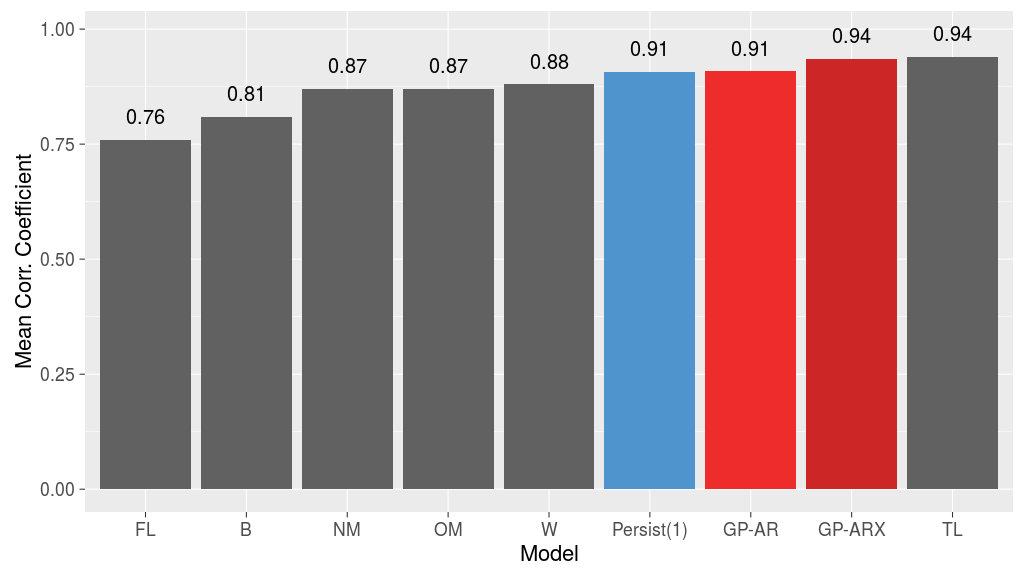
\includegraphics[width=\textwidth]{Compare_CC.png}
      \caption{Averaged cross correlation performance of \emph{GP-AR}, \emph{GP-ARX} and the \emph{Persistence} model versus results in \citet{Ji2012}.}
         \label{fig:cc}
\end{figure}

\subsection{Model Comparison}

Table \ref{table:DstModels} gives a brief enumeration of the models compared. We use the same performance benchmark results published in \citet{Ji2012} and we add the results obtained from testing \emph{GP-AR}, \emph{GP-ARX} as well as the \emph{Persistence} model on the same list of storms. 

For the purpose of generating the cumulative probability plots of the model errors, we need to obtain hourly predictions for all the storm events using the \emph{NARMAX} and \emph{TL} models. In the case of the \emph{NM} model, the formula outlined in \citet{balikhin:narmax} is used to generate hourly predictions. For the \emph{TL} model we use real time predictions listed on their website (\url{http://lasp.colorado.edu/home/spaceweather/}) corresponding to all the storm events. The real time predictions are at a frequency of ten minutes and hourly predictions are generated by averaging the $Dst$ predictions for each hour.

\begin{table}
      \caption[]{One Step Ahead $Dst$ prediction models compared in \citet{Ji2012}}
         \label{table:DstModels}
      
         \begin{tabular}{lll}
            \hline
            \noalign{\smallskip}
            Model  &  Reference  &  Description \\
            \noalign{\smallskip}
            \hline
            \noalign{\smallskip}
            TL & \citet{JGRA:JGRA16300} & Auto regressive model decomposable into additive terms.      \\
            NM & \citet{balikhin:narmax} & Non linear auto regressive with exogenous inputs. \\
            B & \citet{JGR:JGR10260} & Prediction of $Dst$ by solving ODE having injection and decay terms. \\
            W & \citet{Wang:Dst} & Obtained by modification of injection term in \citet{JGR:JGR10260}. \\
            FL & \citet{GRL:GRL11549} & Uses polarity of magnetic clouds to predict geomagnetic response.\\
            OM & \citet{JGRA:JGRA14856} & Modification of injection term in \citet{JGR:JGR10260}.\\
            \noalign{\smallskip}
            \hline
         \end{tabular}
\end{table}

With respect to the \emph{TL} model one important caveat must be noted. The training of the \emph{TL} model was performed on the OMNI data from 1996-2002 which overlaps with a large number of the storm events, therefore the experimental procedure has a strong bias towards \emph{TL} model.

\begin{figure}
   \centering
   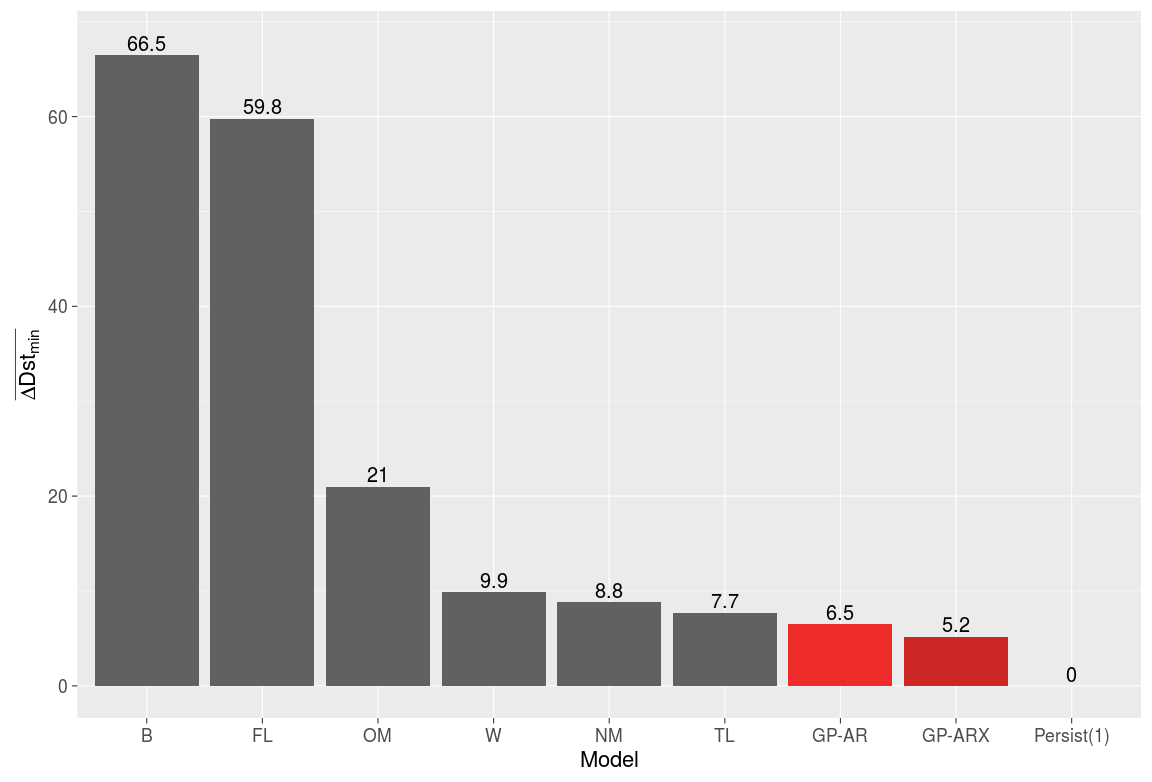
\includegraphics[width=\textwidth]{Compare_deltaDst.png}
      \caption{Averaged $\Delta Dst_{min}$ of \emph{GP-AR}, \emph{GP-ARX} and the \emph{Persistence} model versus results in \citet{Ji2012}.}
         \label{fig:deltaDst}
   \end{figure}

\section{Results} \label{sec:res}

Figures \ref{fig:rmse}, \ref{fig:cc}, \ref{fig:deltaDst} and \ref{fig:timingErr} compare the performance of \emph{GP-AR}, \emph{GP-ARX} and the \emph{Persistence} model with the existing results of \citet{Ji2012}. Figure \ref{fig:rmse} compares the average RMSE of the predictions over the list of 63 storms. One can see that the \emph{GP-ARX} model gives an improvement of approximately $40\%$ in RMSE with respect to the \emph{TL} model and $62\%$ improvement with respect to the \emph{NM} model. It can also be seen that the \emph{Persistence} model gives better \emph{RMSE} performance than the models compared in \citet{Ji2012}.

\begin{figure}
   \centering
   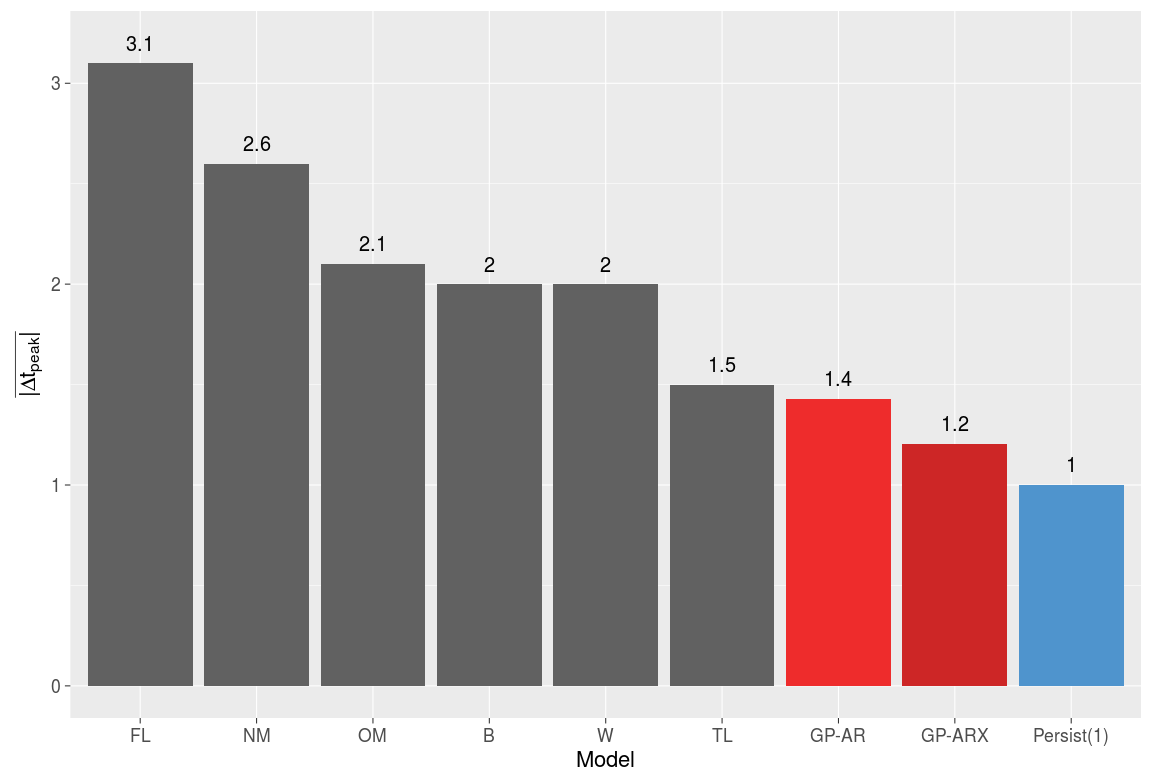
\includegraphics[width=\textwidth]{Compare_timingerr.png}
      \caption{Averaged absolute timing error of \emph{GP-AR}, \emph{GP-ARX} and the \emph{Persistence} model versus results in \citet{Ji2012}.}
         \label{fig:timingErr}
   \end{figure}

Figure \ref{fig:cc} shows the comparison of correlation coefficients between model predictions and actual $Dst$ values. From the results of \citet{Ji2012}, the \emph{TL} model gives the highest correlation coefficient of $94\%$, but that is not surprising considering the fact that there is a large overlap between the training data used to train it and storm events. Even so the \emph{GP-ARX} model gives a comparable correlation coefficient to \emph{TL}, although the training set of the \emph{GP-ARX} model has no overlap with the storm events which is not the case for \emph{TL}.

\begin{figure}
   \centering
   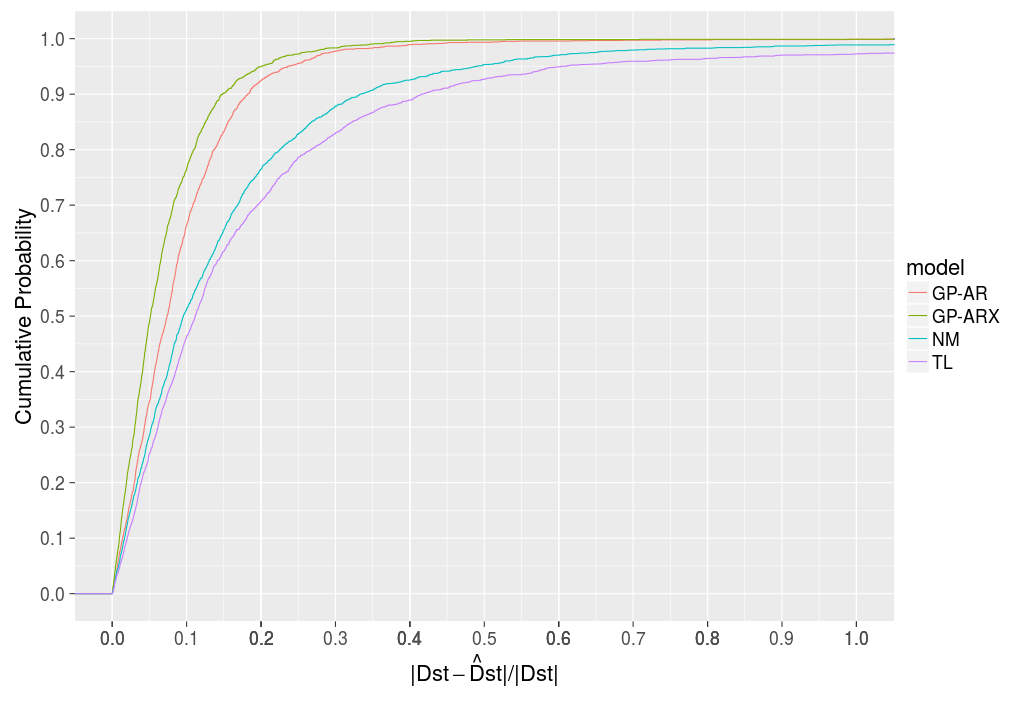
\includegraphics[width=\textwidth]{Compare_RelProb.png}
   \caption{Comparison of empirical distribution of relative errors for \emph{GP-AR}, \emph{GP-ARX}, \emph{NM} and \emph{TL} on the test set of \citet{Ji2012}.}
   \label{fig:relprob}
\end{figure}

Figure \ref{fig:deltaDst} compares the different models with respect to accuracy in predicting the peak value of $Dst$ during storm events ($\Delta Dst_{min}$ averaged over all storms). In the context of this metric the \emph{GP-ARX} model gives a $32\%$ improvement over the \emph{TL} model and $41\%$ over the \emph{NM} model. It is trivial to note that by definition, the \emph{Persistence} model ($\hat{Dst}(t) = Dst(t-1)$) will have $\Delta Dst_{min} = 0$ for every storm event.

Figure \ref{fig:timingErr} compares the time discrepancy of predicting the storm peak. By definition, the \emph{Persistence} model will always have $\Delta t_{peak} = -1$. The \emph{GP-AR} and \emph{GP-ARX} models give better performance than the other models in terms of timing error in prediction of storm peaks. 

\begin{figure}
   \centering
   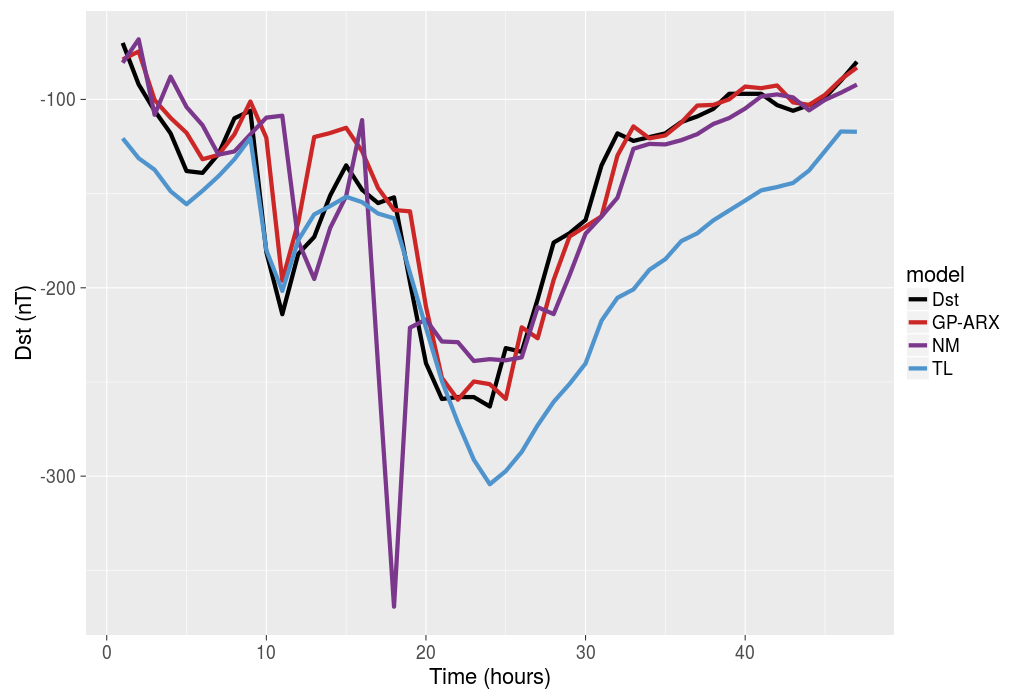
\includegraphics[width=\textwidth]{Compare_pred.png}
      \caption{Comparison of OSA predictions generated by the \emph{NM}, \emph{TL} and \emph{GP-ARX} models for the storm event $9^{th}$ November $2004$ 11:00 UTC - $11^{th}$ November $2004$ 09:00 UTC}
         \label{fig:predictions}
\end{figure}

\begin{figure}
   \centering
   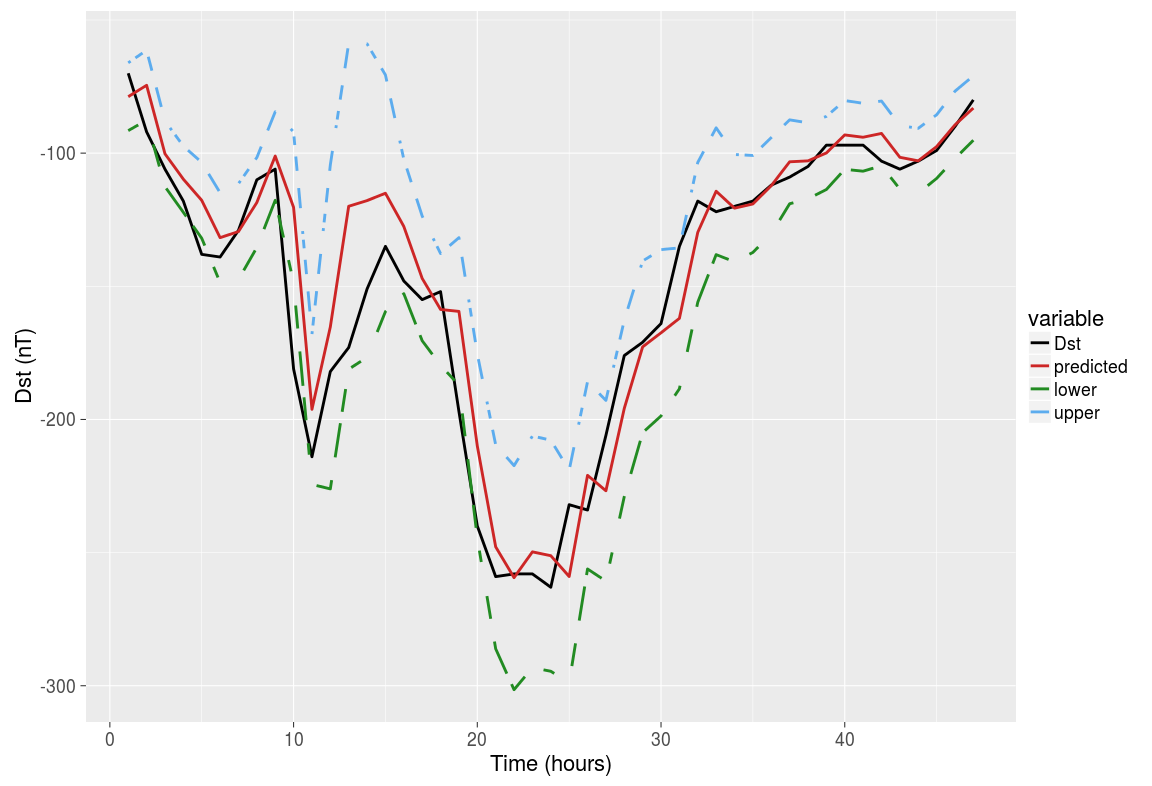
\includegraphics[width=\textwidth]{Compare_pred_err_bar.png}
      \caption{OSA predictions with error bars $\pm 1$ standard deviation, generated by the \emph{GP-ARX} model for the storm event $9^{th}$ November $2004$ 11:00 UTC - $11^{th}$ November $2004$ 09:00 UTC}
         \label{fig:predictionswitherrorbar}
\end{figure}

Figure \ref{fig:relprob} compares the empirical cumulative distribution functions of the absolute value of the relative errors across all storm events in the experiments.  One can see that $95\%$ of the hourly predictions have a relative error smaller than $20\%$ for \emph{GP-ARX}, $50\%$ for \emph{NM} and $60\%$ for \emph{TL}.

In Figure \ref{fig:predictions} we show the OSA predictions generated by the \emph{TL}, \emph{NM} and \emph{GP-ARX} models for one event from the list of storms in \citet{Ji2012}. This storm is interesting due to its strength ($Dst_{min} = -289 \ nT$) and the presence of two distinct peaks. In this particular event the \emph{GP-ARX} model approximates the twin peaks as well as the onset and decay phases quite faithfully, contrary the \emph{NM} and \emph{TL} model predictions. The \emph{TL} model recognises the presence of twin peaks but overestimates the second one as well as the decay phase, while the \emph{NM} model is much delayed in the prediction of the initial peak and fails to approximate the time and intensity of the second peak.

As noted in section \ref{sec:inference}, \emph{Gaussian Process} models generate probabilistic predictions instead of point predictions, giving the modeller the ability to specify error bars on the predictions. In Figure \ref{fig:predictionswitherrorbar}, \emph{OSA} predictions along with lower and upper error bars generated by the \emph{GP-ARX} model are depicted for the event shown in Figure \ref{fig:predictions}. The error bars are calculated at one standard deviation on either side of the mean prediction, using the posterior predictive distribution in equations (\ref{eq:posteriormean}) and (\ref{eq:posteriorcov}). Since the predictive distributions are Gaussian, one standard deviation on either side of the mean corresponds to a confidence interval of $68\%$.



\section{Conclusions}

In this paper, we proposed two \emph{Gaussian Process} auto-regressive models, \emph{GP-ARX} and \emph{GP-AR}, to generate hourly predictions of $Dst$. We compared the performance of our proposed models with the \emph{Persistence} model and six existing model benchmarks reported in \citet{Ji2012}. Predictive performance was compared on \emph{RMSE}, \emph{CC}, $\Delta Dst_{min}$ and $|\Delta t_{peak}|$ calculated on a list of 63 geomagnetic storms from \cite{Ji2012}.

Our results can be summarized as follows.
   \begin{enumerate}
      \item \emph{Persistence} model must be central in the model evaluation process in the context of \emph{one step ahead} prediction of the $Dst$ index. It is clear that the \emph{persistence} behavior in the $Dst$ values is very strong i.e. the trivial predictive model $\hat{Dst}(t) = Dst(t-1)$ gives excellent performance according to the metrics chosen. In fact it can be seen in Figure \ref{fig:rmse} that the \emph{Persistence} model outperforms every model compared by \citet{Ji2012} in the context of OSA prediction of $Dst$. Therefore any model that is proposed to tackle the OSA prediction problem for $Dst$ should be compared to the \emph{Persistence} model and show visible gains above it.
      
      \item \emph{Gaussian Process} AR and ARX models give encouraging benefits in OSA prediction even when compared to the \emph{Persistence} model. Leveraging the strengths of the Bayesian approach, they are able to learn robust predictors from data. 
      
      If one compares the training sets used by all the models, one can appreciate that the models presented here need relatively small training and validations sets: the training set contains 250 instances, while the validation set contains 432 instances. On the other hand the \emph{NM} model uses one year (8760 instances) of data to learn the formula outlined in \citet{balikhin:narmax} and the \emph{TL} model uses six years of data (52560 instances) for training. 
      
      The encouraging results of Gaussian Processes illustrate the strengths of the Bayesian approach to predictive modeling. Since the GP models generate predictive distributions for test data and not just point predictions they lend themselves to the requirements of space weather prediction very well because of the need to generate error bars on predictions.
   \end{enumerate}
   

\begin{acknowledgements}
      We acknowledge use of NASA/GSFC's Space Physics Data Facility's OMNIWeb (or CDAWeb or ftp) service, and OMNI data. We also acknowledge the authors of \citet{JGRA:JGRA16300} for their scientific inputs towards understanding the \emph{TL} model and assistance in access of its generated predictions. Simon Wing acknowledges supports from CWI and NSF Grant AGS-1058456 and NASA Grants (NNX13AE12G, NNX15AJ01G, NNX16AC39G).   
\end{acknowledgements}

%%    This version assumes use of bibtex with the swsc.bib file being present
%%    If your bib file has a different name you need to change the following line

\bibliography{swsc}

%\end{linenumbers}

%\end{document}

%%    If you wish to include your bibliography items in your tex file 
%%    using {thebibliography} as shown below you must out-comment the 
%%    three lines above (insert % at the start of each line) 

%\begin{thebibliography}{}
%\end{thebibliography}

\end{linenumbers}

\end{document}